\documentclass{nuevotema}

\tema{3A-37}
\titulo{Política fiscal. Especial referencia a los efectos sobre el crecimiento económico y el ahorro.}

\begin{document}

\ideaclave

AÑADIR \href{https://voxeu.org/article/fiscal-consolidation-what-speed}{Blanchard y Leigh (2013) -- Debate en VOXEU} y Blanchard y Leigh (2013) (working paper) a descargar de gen.lib.rus.ec.

\seccion{Preguntas clave}

\begin{itemize}
	\item ¿Qué es la política fiscal?
	\item ¿Para qué sirve?
	\item ¿Cuáles son sus efectos?
	\item ¿Qué modelos tratan de explicarlos?
	\item ¿Cómo debe ser la política fiscal?
	\item ¿Qué efectos tiene sobre el crecimiento?
	\item ¿Qué efectos tiene sobre el ahorro?
\end{itemize}

\esquemacorto

\begin{esquema}[enumerate]
	\1[] \marcar{Introducción}
		\2 Contextualización
			\3 Macroeconomía
			\3 Política fiscal
			\3 Estabilización y crecimiento
		\2 Objeto
			\3 ¿Qué es la política fiscal?
			\3 ¿Para qué sirve?
			\3 ¿Puede la política fiscal estabilizar una economía
			\3 ¿Cuáles son sus efectos?
			\3 ¿Qué modelos tratan de explicarlos?
			\3 ¿Cómo debe ser la política fiscal?
			\3 ¿Qué efectos tiene sobre el crecimiento?
			\3 ¿Qué efectos tiene sobre el ahorro?
		\2 Estructura
			\3 La política fiscal estabilizadora
			\3 Efectos sobre el crecimiento y el ahorro
	\1 \marcar{La política fiscal estabilizadora}
		\2 Idea clave
			\3 Contexto
			\3 Objetivos
			\3 Resultados
		\2 Instrumentos de política fiscal
			\3 Tributación
			\3 Gasto público
			\3 Estabilizadores automáticos
			\3 Tono de la política fiscal
		\2 Modelo clásico
			\3 Idea clave
			\3 Papel muy limitado de la política fiscal
			\3 Valoración
		\2 Modelo neoclásico
			\3 Idea clave
		\2 Modelo keynesiano
			\3 Idea clave
			\3 Formulación
			\3 Implicaciones
		\2 Síntesis neoclásica
			\3 Idea clave
			\3 Formulación
			\3 Implicaciones
			\3 Valoración
		\2 Mundell-Fleming
			\3 Idea clave
			\3 Formulación
		\2 Monetarismo
			\3 Idea clave
			\3 Formulación
			\3 Implicaciones
			\3 Valoración
		\2 Nueva Macroeconomía Clásica
			\3 Idea clave
			\3 Formulación
			\3 Implicaciones
			\3 Valoración
		\2 Modelo del ciclo real
			\3 Idea clave
			\3 Formulación
			\3 Implicaciones
			\3 Valoración
		\2 Modelos neo-keynesianos de segunda generación
			\3 Idea clave
			\3 Formulación
			\3 Implicaciones
			\3 Retardos
			\3 Gastos comprometidos
		\2 Evidencia empírica
			\3 Métodos de estimación
			\3 Equivalencia ricardiana
			\3 Multiplicadores
			\3 Factores coyunturales
			\3 Importancia de la previsión
			\3 Consolidaciones expansivas
			\3 Estabilizadores automáticos
	\1 \marcar{Efectos sobre el crecimiento y el ahorro}
		\2 Ahorro
			\3 Idea clave
			\3 Formulación básica (sin sistema de pensiones)
			\3 Sistema de capitalización
			\3 Sistema pay-as-you-go / PAYG
			\3 Comparación sistemas capitalizados vs PAYG
			\3 Extensiones
		\2 Crecimiento
			\3 Idea clave
			\3 Crecimiento exógeno
			\3 Crecimiento endógeno con gasto público improductivo
			\3 Crecimiento endógeno con gasto público productivo
	\1 \marcar{Conclusión}
		\2 Recapitulación
			\3 La política fiscal estabilizadora
			\3 Efectos sobre el crecimiento y el ahorro
		\2 Idea final
			\3 Crisis financiera y política fiscal
			\3 Unión Europea y política fiscal
			\3 Envejecimiento de la población

\end{esquema}

\esquemalargo













\begin{esquemal}
	\1[] \marcar{Introducción}
		\2 Contextualización
			\3 Macroeconomía
				\4 Análisis de fenómenos económicos a gran escala
				\4 Énfasis sobre variables agregadas
			\3 Política fiscal
				\4 Conjunto de actuaciones del sector público
				\4[] Por el lado del ingreso
				\4[] $\to$ Impuestos y cotizaciones
				\4[] Por el lado del gasto
				\4[] $\to$ Gasto corriente
				\4[] $\to$ Inversión pública
				\4[] $\to$ Subsidios y subvenciones
				\4[] $\to$ Pensiones
				\4[$\to$] Con incidencia sobre:
				\4[] Demanda agregada
				\4[] Stock de capital
				\4[] Consumo privado
				\4[] Deuda pública
				\4[] Tipo de interés
				\4 Relevancia de la política fiscal
				\4[] Gasto público cercano al 40\% en Europa
				\4[] Elemento central de tres funciones del sector público
				\4[] $\to$ Asignación
				\4[] $\to$ Estabilización
				\4[] $\to$ Redistribución
				\4[] Políticas fiscales en crisis
				\4[] $\to$ New Deal tras Gran Depresión
				\4[] $\to$ Aumento del gasto consolidado tras IIGM
				\4[] $\to$ Estado del Bienestar en Europa
				\4[] $\to$ + gasto y -- recaudación tras crisis 2008
				\4[] $\to$ Crisis de deuda posterior
				\4[] $\then$ Efectos sobre output en c/p y crecimiento de l/p
			\3 Estabilización y crecimiento
				\4 Estabilización
				\4[] Reducir las amplitud de fluctuaciones de VAgregadas
				\4 Crecimiento
				\4[] Aumento del output per cápita en el largo plazo
				\4 Política fiscal afecta a ambos
				\4[] Aspectos objetivos esenciales de policy-maker
		\2 Objeto
			\3 ¿Qué es la política fiscal?
			\3 ¿Para qué sirve?
			\3 ¿Puede la política fiscal estabilizar una economía
			\3 ¿Cuáles son sus efectos?
			\3 ¿Qué modelos tratan de explicarlos?
			\3 ¿Cómo debe ser la política fiscal?
			\3 ¿Qué efectos tiene sobre el crecimiento?
			\3 ¿Qué efectos tiene sobre el ahorro?
		\2 Estructura
			\3 La política fiscal estabilizadora
			\3 Efectos sobre el crecimiento y el ahorro
	\1 \marcar{La política fiscal estabilizadora}
		\2 Idea clave
			\3 Contexto
				\4 Sector público controla \% de VAB
				\4 Economías sufren fluctuaciones cíclicas
				\4[] Evidencia empírica consistente
			\3 Objetivos
				\4 Reducir fluctuaciones cíclicas de output y empleo
				\4 Maximizar utilización de capacidad productiva
			\3 Resultados
				\4 Multiplicador fiscal
				\4[] Impacto de corto plazo de un shock de PF
				\4[] $\to$ Ratio de cambio en output vs déficit respecto base
				\4[] $\then$ Elemento central a estimar en PF
				\4[] $\then$ Papel clave para diseño de política fiscla
		\2 Instrumentos de política fiscal
			\3 Tributación
				\4 Ingresos coactivos del sector público con origen en SP
			\3 Gasto público
				\4 Demanda de bienes y servicios por sector público
				\4 Diferentes categorías en términos de CN
				\4[] Operaciones financieras
				\4[] Operaciones no financieras
				\4[] $\to$ Capital
				\4[] $\to$ Corriente
				\4 Gasto no financiero
				\4[] $\to$ Relevante a efectos de PF estabilizadora
				\4[] $\to$ Operaciones financieras no afectan DA directamente
			\3 Estabilizadores automáticos
				\4 Instrumentos de gasto y tributación
				\4 No requieren actuación discrecional
				\4 Ejemplos
				\4[] Subsidios por desempleo
				\4[] $\to$ $\uparrow$ trans. cuando aumenta paro
				\4[] Fiscalidad progresiva
				\4[] $\to$ $\uparrow$ presión fiscal cuando $\uparrow$ renta
			\3 Tono de la política fiscal\footnote{Ver \textit{fiscal stance} en Palgrave.}
				\4 Varias definiciones
				\4 Inicialmente
				\4[] En relación a saldo público en pleno empleo
				\4[] $\to$ Superávit en pleno empleo $\to$ PF contractiva\\
				\4[] $\to$ Déficit en pleno empleo $\to$ PF expansiva
				\4 Posteriormente
				\4[] Aparición de nuevos conceptos
				\4[] $\to$ ``Desempleo de equilibrio''
				\4[] $\to$ Desempleo persistente
				\4[] $\to$ Output gap
				\4[] Definición de tono de PF respecto output gap
				\4 Representación gráfica
				\4[] \grafica{tonopf}
		\2 Modelo clásico
			\3 Idea clave
				\4 Contexto
				\4 Objetivos
				\4 Resultados
			\3 Papel muy limitado de la política fiscal
				\4 Economía tiende a estabilidad por sí misma
				\4[] Mecanismos de ajuste hacia pleno empleo
				\4[] Ley de Say se cumple en el corto plazo
				\4[$\then$] Sin apenas papel estabilizador para política fiscal
				\4[$\then$] Limitada a funciones concretas
				\4[] $\to$ Fundamentalmente, suplir fallos de mercado
				\4[] $\to$ Construcción de trabajos públicos
				\4[] $\to$ Defensa, orden justicia
				\4[] $\to$  Educación básica
				\4[$\then$] Lado del ingreso debe respetar ciertos principios
				\4[] Principios básicos de la tributación
				\4[] $\to$ GEFCESS\footnote{Generalidad, eficiencia, flexibilidad, continuidad, equidad, suficiencia, sencillez administrativa. Ver tema 4B-8.}
				\4[$\then$] Debate sobre cómo implementar política fiscal
				\4[] Gasto público debe financiarse
				\4[] ¿Cómo hacerlo?
			\3 Valoración
				\4 Visión consolidada hasta Gran Depresión
				\4[] Gasto público debe mantenerse pequeño
				\4[] Cuentas públicas deben equilibrarse
				\4[] Estabilización vía política fiscal no es deseable
				\4 Algunas discrepancias
				\4[] Malthus
				\4[] $\to$ Ley de Say no siempre se cumple
				\4[] $\then$ Rentistas e improductivos aumenta DAgregada
				\4[] Stuart Mill
				\4[] $\to$ Política fiscal puede alterar distribución
				\4[] $\to$ Distribución y producción interaccionan
				\4[] $\to$ Análisis de progresividad
				\4[] Hobson
				\4[] $\to$ Subconsumo es posible
				\4[] $\to$ Desempleo persistente es posible
				\4[] $\to$ Exceso de ahorro posible
				\4[] $\to$ Redistribución del ingreso vía fiscal posible
		\2 Modelo neoclásico
			\3 Idea clave
				\4 Contexto
				\4[] Fisher, Wicksell, Pigou...
				\4[] Treasury View
				\4[] Austriacos
				\4[] Keynes recopila visión neoclásica
				\4[] $\to$ Realmente, denomina clásica
				\4 Objetivo
				\4[] Servir de modelo de comparación con Keynes
				\4 Implicaciones
				\4[] Política fiscal no afecta DA ni empleo
				\4[] Sólo puede hacer crowding-out de inversión
				\4[] Flexibilización de mercado de trabajo para $\downarrow$ empleo
				\4[] $\to$ No política fiscal
				\4 Formulación
				\4 Output determinado en mercado de trabajo
				\4[] $\to$ Mercado perfectamente competitivo
				\4[] $\to$ Salario real se ajusta para eq. oferta y demanda
				\4[] $\then$ Output determinado por
				\4 Equilibrio de demanda agregada:
				\4[] $\to$ $C+I(r) + G = C + S + T$
				\4[] $\then$ $S - I(r) = G-T$
				\4 Implicaciones
				\4[] Aumento demanda agregada vía política fiscal
				\4[] $\to$ No aumenta output
				\4[] $\to$ Reduce inversión privada
		\2 Modelo keynesiano
			\3 Idea clave
				\4 Demanda agregada determina output y empleo
				\4 Política fiscal afecta demanda agregada
				\4[] $\then$ Política fiscal herramienta esencial de PEconómica
			\3 Formulación
				\4 Demanda agregada
				\4[] $\to$ Consumo: autónomo y en función de renta
				\4[] $\to$ Inversión: depende de interés
				\4[] $\to$ Gasto público exógno
				\4 Oferta agregada
				\4[] $\to$ Exceso de capacidad productiva
				\4[] $\then$ Aumenta con demanda agregada
				\4[] $\then$ Inflación posterior
			\3 Implicaciones
				\4 Política fiscal puede aumentar output
				\4[] Economía no tiende a plena utilización de capacidad
				\4[] $\to$ Rigideces nominales y reales
				\4[] $\to$ Poder de mercado en bienes
				\4[] $\to$
				\4[] $\then$
				\4 Posibles múlt. equilibrios con exceso de capacidad
				\4[] $\to$ Capital y trabajo sin utilizar
				\4[] $\then$ Desempleo
				\4[] Política fiscal puede inducir equilibrio
				\4[] $\to$ Con más renta
				\4[] $\to$ Con menos desempleo
				\4 Efecto multiplicador del gasto público
				\4[] Aumentos del gasto público aumentan renta > 1:1
				\4[] $Y = C_0 + c Y + G_0$
				\4[] $\then$ $Y = \frac{C_0 + G_0}{1-c}$
				\4 Déficit fiscales son herramienta principal
				\4[] En recesión, capacidad productiva sin utilizar
				\4[] Déficits fiscales estimulan demanda agregada
				\4[] $\to$ Aumentar gasto
				\4[] $\to$ Reducir
				\4 PM pasiva para mantener interés bajo
		\2 Síntesis neoclásica
			\3 Idea clave
				\4 Contexto
				\4[] Análisis keynesiano paradigma dominante
				\4[] Éxito de políticas keynesianas en años 30, 40, 50s
				\4[] Formulación matemática y diagramática
				\4[] Marco IS-LM
				\4[] Tensión entre modelo clásico y keynesiano
				\4 Objetivo
				\4[] Reconciliar modelo clásico y keynesiano
				\4[] Efectos de política fiscal en corto y largo plazo
				\4 Resultados
				\4[] Análisis de PF diferenciado
				\4[] $\to$ Entre c/p y l/p
				\4[] Modelo matemático simple de economía
				\4[] $\to$ Ligero cambio en supuestos cambia resultados
			\3 Formulación
				\4 Marco IS-LM
				\4 IS: $Y = C_0 + c(y(1-t)+\text{TR})+I(r) + G$
				\4 LM: $\frac{M}{P} = L(y,r)$
				\4 Multiplicador del gasto público
				\4[] $\frac{d Y}{d G} = \frac{1}{1-c(1-t) + I_i \frac{L_Y}{L_i}}$
				\4 Multiplicador de las transferencias
				\4[] $\frac{d Y}{d \text{TR}} = \frac{c}{1-c(1-t) + I_i \frac{L_Y}{L_i}}$
				\4 Multiplicador de los impuestos
				\4[] Tomando $T=t\cdot y$
				\4[] $\frac{d Y}{d T} = \frac{-c}{1-c(1-t) + I_i \frac{L_Y}{L_i}}$
			\3 Implicaciones
				\4 Interacción con PF con demanda de dinero
				\4[] Cuanto mayor sensibilidad dda. dinero a Y
				\4[] $\to$ Más debe aumentar interés para eq. en mercado dinero
				\4[] $\to$ Más caída de inversión
				\4[] $\then$ Menor efecto multiplicador
				\4[]  Cuanto mayor sensibilidad dda. dinero a r
				\4[] $\to$ Mayor efecto multiplicador
				\4 Interacción con interés
				\4[] Cuanto mayor sensibilidad de inversión a interés
				\4[] $\to$ Menor efecto multiplicador
				\4[] $\then$ Crowding-out de inversión
				\4 Aumento del gasto manteniendo equilibrio presupuestario
				\4[] Suma de efectos de aumento de gasto e impuestos
				\4[] $\frac{d Y}{d G} \cdot d G + \frac{d Y}{d T} \cdot d T = \frac{1-c}{1-c(1-t) + I_i \frac{L_Y}{L_i}}$
				\4[$\then$] Efecto positivo dados supuestos
				\4[$\then$] No se ha considerado exceso de gravamen
				\4 Política fiscal estabilizadora
				\4[] En recesión
				\4[] $\to$ Política fiscal expansiva
				\4[] $\then$ Aumento del gasto
				\4[] $\then$ Bajada de impuestos
				\4[] En crecimiento
				\4[] $\to$ Política fiscal contractiva
				\4[] $\then$ Reducción del gasto
				\4[] $\then$ Aumento de impuestos
				\4[] Política monetaria pasiva
				\4[] Mantener tipos de interés bajos
				\4[] $\then$ Functional finance
				\4 Economía abierta
				\4[] Estímulo de DA parcialmente a importaciones
				\4[] Parte del efecto se expansivo se ``filtra'' a exterior
				\4 Stock de deuda
				\4[] Modelo anterior no contempla
				\4[] $\to$ Posible cumplimiento de equivalencia ricardiana
				\4[] Aumento del déficit público
				\4[] $\to$ Puede inducir caída de la demanda privada
				\4[] $\then$ Agentes estiman subida futura de impuestos
				\4[] $\then$ Agentes ahorran ahora para pagar impuestos futuros
			\3 Valoración
				\4 Marco de análisis flexible
				\4[] Cambio parsimonioso en supuestos
				\4[] $\to$ Permite modelizar diferentes efectos
				\4 PF es principal herramienta de política económica
				\4 Predomina en 50s y 60s
				\4 Formulación en marco IS-LM
				\4[] Dos ecuaciones, dos incógnitas
				\4[] $\to$ Y, r
				\4[] $\to$ Precios exógenos $\to$ Curva de Phillips
				\4 Dicotomía largo-corto plazo
				\4[] En corto plazo, economía keynesiana
				\4[] A largo plazo, economía clásico
		\2 Mundell-Fleming
			\3 Idea clave
				\4 Contexto
				\4[] Macroeconomías abiertas
				\4[] $\to$ Comercio exterior
				\4[] $\to$ Flujos de capital
				\4[] Políticas macroeconómicas
				\4[] $\to$ Alteran flujos exteriores
				\4[] Flujos exteriores
				\4[] $\to$ Afectan efectos de políticas macro
				\4 Objetivo
				\4[] Efectos de políticas macroeconomías
				\4[] Efectos de política fiscal
				\4[] $\to$ En economías abiertas
				\4 Resultados
				\4[] Efectividad de PF depende de régimen exterior
				\4[] PF efectiva aumentando output
				\4[] $\to$ Movilidad de capital+TCN Fijo
				\4[] $\to$ Sin mov. de K+TCN Flexible
			\3 Formulación
				\4 Extensión de análisis IS-LM a economía abierta
				\4[] IS: $Y = C_0 + cY + I(r) + \text{NX}(Y,e)$
				\4[] LM: $\frac{M}{P} = L(Y,r)$
				\4[] BP: $\Delta R = \text{NX} (Y,e) - \text{CF}(r-r^*)$
				\4 Política fiscal puede ser efectiva
				\4[] Depende del régimen cambiario y movimiento de K
				\4 PF efectiva: Libre mov. de K + TCFijo
				\4[] $\to$ PF $\uparrow$ Y, $\uparrow$ r
				\4[] $\to$ $r > r^*$ $\then$ ENeta de Capital
				\4[] $\then$ Presión a apreciación y reducción NX
				\4[] $\then$ PM para mantener $r=r^*$
				\4[] $\then$ Aumento Y, $r = r^*$
				\4 PF efectiva: Sin movilidad de K +  TCFlexible
				\4[] $\to$ PF $\uparrow$ Y, $\downarrow$ NX
				\4[] $\to$ $\Delta R = 0$, $\text{CF} = 0$
				\4[] $\then$ Exceso de oferta de moneda local
				\4[] $\then$ Depreciación del tipo de cambio
				\4[] $\then$ $\uparrow NX$
				\4[] $\then$ Efecto global positivo sobre DA y output
				\4 PF inefectiva con:
				\4[] Libre movimiento de K +TCN flexible
				\4[] $\to$ PF provoca aumento de interés
				\4[] $\to$ Entradas de capital aprecian moneda
				\4[] $\then$ Apreciación reduce exportaciones netas
				\4[] $\then$ IS a la izquierda hasta eliminar divergencia de interés
				\4[] Sin movimiento de capital+TCN fijo
				\4[] $\to$ PF provoca exceso de demanda de divisas
				\4[] $\then$ Venta de divisa contrae oferta monetaria
				\4[] $\then$ LM se desplaza hacia izquierda
				\4[] $\then$ Vuelta a output inicial con más interés, menos reservas
		\2 Monetarismo
			\3 Idea clave
				\4 Contexto
				\4[] Neutralidad monetaria de largo plazo
				\4[] Dinero no neutral en corto plazo
				\4[] Velocidad del dinero
				\4[] $\to$ Debate sobre estabilidad
				\4[] $\to$ Monetaristas afirman estabilidad inherente
				\4[] $\then$ Dda. dinero poco elástica a interés monetario
				\4[] $\then$ LM pendiente muy elevada
				\4 Objetivo
				\4[] Comparar efectos de PM con PF
				\4 Resultados
				\4[] PF poco efectiva
				\4[] Sujeta a lags
				\4[] Demanda de dinero
			\3 Formulación
				\4 Multiplicador del gasto muy bajo
				\4[] Hogares deciden consumo en función de renta permanente
				\4[] $\to$ No de renta presente
				\4[] Expansiones fiscales transitorias
				\4[] $\to$ Apenas aumentan renta permanente
				\4[] $\then$ Poco efecto sobre output
				\4 Demanda de inversión
				\4[] Muy sensible a interés
				\4[] Déficit público a oferta monetaria constante
				\4[] Aumento del tipo de interés
				\4[] $\then$ Demanda agregada apenas aumenta
				\4 Demanda de dinero
				\4[] Sensible a muchos factores aparte de $r$ e $y$
				\4[] $\to$ Interés de activos de largo plazo
				\4[] $\to$ Riqueza permanente
				\4[] Aumento de renta con oferta monetaria constante
				\4[] $\to$ Requiere fuerte aumento de interés monetario
				\4[] $\then$ Caída de inversión
				\4 Canal indirecto/keynesiano de PM muy fuerte
				\4[] A diferencia de Keynes
				\4[] $\then$ Crowding-out potencial mayor de $\downarrow$DA
			\3 Implicaciones
				\4 PF poco efectiva estimulando DA
				\4[] Poco efecto multiplicador
				\4[] Crowding-out
				\4 PM preferible
				\4[] Aunque genera otros problemas
			\3 Valoración
				\4 Inversión muy sensible al tipo de interés
				\4[] Aumento del déficit público
				\4[] $\to$ Aumento del interés
				\4[] $\then$ Crowding-out de inversión privada
				\4[] $\then$ Inversión total cae/aumenta poco
				\4 Política monetaria es principal causante de ciclo
				\4[] Vía rigideces reales
				\4[] Pero no puede utilizarse como estímulo permanente
				\4[] $\to$ Espiral inflacionaria
				\4 Régimen de política económica es relevante
				\4[] Política discrecional es contraproducente
		\2 Nueva Macroeconomía Clásica
			\3 Idea clave
				\4 Contexto
				\4[] HER
				\4[] $\to$ Agentes estiman eficientemente dada información
				\4[]
				\4 Objetivos
				\4 Resultados
			\3 Formulación
				\4 Microfundamentación+HER
				\4[] Macroeconomía como equilibrio general walrasiano
				\4[] $\to$ De agentes racionales optimizadores
				\4[] $\to$ Hipótesis de Expectativas racionales
				\4 Economías tienden a equilibrio continuo
				\4[] $\to$ Política económica es inefectiva e innecesaria
				\4[] $\to$ Monetaria y fiscal
				\4 Equivalencia ricardiana reformulada por Barro
				\4[] ¿La deuda pública es riqueza neta?
				\4[] $\to$ ¿Aumenta riqueza neta financiando gasto con bonos?
				\4[] Agentes consideran renta intertemporal
				\4[] Aumento del gasto público tiene = efectos
				\4[] $\to$ Se financie con deuda o mediante impuestos
				\4[] Necesarios supuestos restrictivos:
				\4[] $\to$ Impuestos de suma fija
				\4[] $\to$ Agentes con vida infinita o altruismo intergeneracional
				\4[] $\to$ Mercados de capital perfectos
				\4[] $\then$ Enmarca problema
				\4[] $\then$ Permite caracterizar razones de incumplimiento
			\3 Implicaciones
				\4 Modelos fundamentan equivalencia ricardiana
				\4[] Financiación del gasto público no tiene efecto
				\4[] Tamaño del gasto público sí tiene efectos
			\3 Valoración
				\4 Poca atención a política fiscal
				\4 Recuperación de conclusiones de clasicismo
				\4[] Papel restringido del estado
		\2 Modelo del ciclo real\footnote{Ver Sims (2017)}
			\3 Idea clave
				\4 Contexto
				\4[] Modelos de NMC
				\4[] $\to$ Macroeconomía es equilibrio general walrasiano
				\4[] Crítica de Lucas
				\4[] $\to$ Microfundamentación para tratar de evitar
				\4[] Modelo neoclásico de crecimiento
				\4[] $\to$ Referencia básica
				\4 Objetivo
				\4[] Valorar efecto de shock de gasto de público
				\4[] $\to$ Considerando optimización racional intertemporal
				\4[] Valorar efectos de shocks de gasto público sobre:
				\4[] $\to$ Consumo
				\4[] $\to$ Trabajo
				\4[] $\to$ Inversión
				\4[] $\to$ Interés
				\4 Resultados
				\4[] Consolidación de marco DSGE
				\4[] $\to$ iniciado por Lucas 1972
				\4[] optimización Dinámica de los agentes
				\4[] sujetos a impulsos eStocásticos
				\4[] en contexto de Equilibrio General
				\4[] Marco de modelización general
				\4[] $\to$ Permite muy numerosas adaptaciones
				\4[] Shocks de gasto público tienen efectos
				\4[] $\to$ Sobre output
				\4[] $\to$ Sobre empleo
				\4[] $\to$ Sobre interés
				\4[] $\to$ Sobre inversión
				\4[] Transitoriedad de shock de gasto es relevante
				\4[] Shocks transitorios
				\4[] $\to$ Puede afectar en mayor medida a ahorro e inversión
			\3 Formulación
				\4 Maximización de los beneficios de las empresas
				\4[] Decidiendo sobre:
				\4[] $\to$ Capital
				\4[] $\to$ Trabajo
				\4[] $\underset{N_t, K_t}{\max} \quad \Pi_t = \underbrace{A_t K_t^\alpha N_t^{1-\alpha}}_{Y_t} - w_t N_t - R_t K_t$
				\4[] CPO: \quad $w_t = (1-\alpha) A_t K_t^\alpha N_t^\alpha$
				\4[] \quad \quad $R_t = \alpha A_t K_t^{\alpha-1} N_t^{1-\alpha}$
				\4[] Donde:
				\4[] $\to$ $A_t = (1-\rho)A + \rho_A A_{t-1} + \epsilon_t$
				\4 Maximización de la utilidad de los consumidores
				\4[] Decidiendo sobre:
				\4[] $\to$ Consumo en periodo
				\4[] $\to$ Trabajo en periodo
				\4[] $\to$ Capital en periodo
				\4[] $\to$ Inversión en activo del gobierno en periodo
				\4[] $\underset{C_t, N_t,K_t, B_t}{\max} \quad \sum_{t=0}^\infty \beta^t u(C_t, N_t)$
				\4[] $\text{s.a}: \quad C_t+\underbrace{K_t - (1-\delta)K_{t-1}}_{I_t} + B_t - (1+r_{t-1})B_{t-1} \leq$
				\4[] \quad \quad \quad $\leq \underbrace{wN_t + R_t K_t + \Pi_t}_{Y_t} - T_t$
				\4[] \quad \quad \quad $\lim_{T \to \infty}  K_t \geq 0$
				\4[] \quad \quad \quad $\then$ $\sum_{t=0}^\infty \frac{C_t + I_t}{(1+r)^t} = \sum_{t=0}^\infty \frac{ Y_t}{(1+r)^{-t}} - \sum_{t=0}^\infty \frac{T_t}{(1+r)^{-t}}$
				\4[] Donde:
				\4[] $\to$ $u(C_t, N_t) = \left( \ln C_t  - v(N_t) \right)$
				\4[] CPO: \quad $u'(C_t) = \beta u'(C_{t+1})$
				\4[] \quad \quad $w_t = \frac{u_{N_T}}{u_{C_t}}$
				\4 Senda exógena de gasto público sujeta a restricción
				\4[] $G_t + r_{t-1} D_t \leq T_t + D_{t+1} - D_t$
				\4[] $\to$ $T_t = G_t - \left( D_t - (1+r_{t-1} D_{t-1}) \right)$
				\4[] Condición de No-Ponzi + Transversalidad
				\4[] $\then$ $\sum_{t=0}^\infty G_t \cdot \frac{1}{(1+r)^t} = \sum_{t=0}^\infty T_t \cdot \frac{1}{(1+r)^t}$
				\4 Resolución por método de Lagrange
				\4[] Si secuencia de shocks es conocida
				\4[] $\to$ $\epsilon_t$ a productividad
				\4[] $\to$ $G_t$ a gasto público
				\4 Resolución por programación dinámica
				\4[] Si shocks aleatorios
				\4 Dinámica del equilibrio
				\4[] $u'(C_t) = \beta u'(C_{t+1})$
				\4[] $w_t = \frac{u_{N_T}}{u_{C_t}}$
				\4[] $C_t + I_t + G_t = Y_t$
				\4[] $I_t = K_{t+1} - (1-\delta) K_t$
				\4[$\then$] Estado estacionario: secuencias de vars. exógenas
				\4[] $C_t = C(K_t, \left\lbrace A_t \right\rbrace^\infty_0, \left\lbrace G_t \right\rbrace )$
				\4[] $N_t = N(K_t, \left\lbrace A_t \right\rbrace^\infty_0, \left\lbrace G_t \right\rbrace )$
				\4[] $K_t = K (K_t, \left\lbrace A_t \right\rbrace^\infty_0, \left\lbrace G_t \right\rbrace )$
				\4 Aproximación y log-linearización
				\4[] Solución suele tomar forma de
				\4[] sistema de eqs. parciales diferenciales
				\4[] $\to$ Sin solución analítica en forma cerrada
				\4[] $\to$ Aproximación de la solución y linearización
				\4 Ecuaciones de dinámica aproximada
				\4[] Tras linearización del estado estacionario
				\4[] $\tilde{C}_{t+1} = a_{CK}\tilde{K}_{t+1} + a_{CA}\tilde{A}_{t+1} + a_{CG} \tilde{G}_{t+1}$
				\4[] $\tilde{L}_{t+1} = a_{LK}\tilde{K}_{t+1} + a_{LA}\tilde{A}_{t+1} + a_{LG} \tilde{G}_{t+1}$
				\4[] $\tilde{K}_{t+1} = b_{KK}\tilde{K}_{t} + b_{KA}\tilde{A}_{t} + b_{KG} \tilde{G}_{t}$
				\4 Parámetros de las ecuaciones de dinámica
				\4[] Derivados de parámetros estructurales exógenos
				\4[] Entre ellos:
				\4[] $\alpha$: elasticidad-capital del output
				\4[] $g$: tasa de crecimiento tendencial
				\4[] $\rho$: tasa de descuento de la utilidad
				\4[] $\rho_\theta$: persistencia del shock de productividad
				\4[] tipo de interés de equilibrio
				\4[] etc...
				\4 Shocks tecnológicos
				\4[] Pueden representar perturbaciones sobre:
				\4[] $\to$  Productividad
				\4[] $\to$ Liberalización y desregulación
				\4[] $\to$ Desastres naturales o guerras
				\4 Filtros de tendencias
				\4[] Métodos matemáticos para extraer
				\4[] $\to$ Componente cíclico
				\4[] $\then$ Shocks de productividad
				\4 Estimados mediante diferentes filtros
				\4[] Descomponer tendencia+ciclo
				\4[] Univariables
				\4[] $\to$ A partir de una variable
				\4[] $\to$ Generalmente, PIB
				\4[] Multivariables
				\4 Filtro de Hodrick-Prescott
				\4[] Hallar secuencia de output tendencia
				\4[] $\to$ Que minimiza función de pérdida
				\4[] Función de pérdida penaliza de:
				\4[] $\to$ Diferencia entre output y tendencia
				\4[] $\to$ Variaciones entre periodos de tendencia
				\4[] $\then$ Parametrizable para variar peso de uno y otro
				\4[] Dibujar gráfica $y$--$t$ y tendencia superpuesta
				\4[] $\tilde{C}_t$, $\tilde{K}_{t+1}$, $\tilde{N}_t$
				\4[] $\to$ Expresan diferencias frente a tendencia
			\3 Implicaciones
				\4 Efectos generales del gasto público
				\4[] Reducción de riqueza disponible
				\4[] Posible efecto sobre utilidad y producción
				\4[] $\to$ Provisión de gasto público
				\4 Shock transitorio de gasto público improductivo
				\4[] Supuestos:
				\4[] $\to$ Gasto público improductivo
				\4[] $\to$ Impuesto de suma fija no distorsionante
				\4[] Output aumenta
				\4[] $\to$ Aunque mucho menos que gasto público
				\4[] Consumo cae
				\4[] $\to$ Muy ligeramente
				\4[] Inversión cae
				\4[] $\to$ Caída muy pronunciada y recuperación rápida
				\4[] Trabajo aumenta
				\4[] $\to$ Muy ligeramente
				\4[] $\to$ Sin efecto sustitución ocio-consumo
				\4[] $\to$ Pequeño efecto renta
				\4[] Salarios caen
				\4[] $\to$ Muy ligeramente
				\4[] $\to$ Aumento de oferta de trabajo
				\4[] $\to$ Menos capital
				\4[] $\to$ Igual productividad
				\4[] Tipo de interés
				\4[] $\to$ Aumenta muy ligeramente
				\4[] Representación gráfica
				\4[] \grafica{rbcefectodynaregastotransitorio}
				\4 Shock permanente del gasto público improductivo
				\4[] Supuestos:
				\4[] $\to$ gasto público improductivo
				\4[] $\to$ Impuesto de suma fija no distorsionante
				\4[] Output aumenta
				\4[] $\to$  Más que con shock transitorio
				\4[] Consumo cae
				\4[] $\to$ Más que con shock transtorio
				\4[] $\to$ Inversión cae
				\4[] $\to$ Más que con shock transitorio
				\4[] $\to$ De manera más persistente
				\4[] Trabajo aumenta
				\4[] $\to$ Más que con shock transitorio
				\4[] $\to$ Efecto renta mucho mayor ahora
				\4[] $\to$ Sin efecto sustitución ocio-consumo
				\4[] Salarios caen
				\4[] $\to$ Más que en transitorio
				\4[] $\to$ Aumento de la oferta de trabajo
				\4[] $\to$ Menos capital
				\4[] $\to$ Igual productividad
				\4[] Tipo de interés
				\4 Representación gráfica
				\4[] \grafica{rbcefectodynaregastopermanente}
				\4 Comparación transitorio-permanente en gasto público
				\4[] Cuanto más persistente sea el shock:
				\4[Consumo] + $\uparrow$ sobre consumo
				\4[Trabajo] + aumento del trabajo
				\4[Salarios] + $\downarrow$ los salarios
				\4[Output] + aumenta el output
				\4[Inversión] + persistente caída de la inversión
				\4[Tipo de interés] + $\uparrow$ el tipo de interés
				\4 Aumento permanente del gasto público productivo
				\4[] Asumiendo
				\4[] $\to$ Impuesto de suma fija
				\4[] $\to$ Distorsión evita inversión óptima
				\4[] Modelos RBC modificados con gasto público productivo
				\4[] $\to$ Gasto público puede dedicarse a inversión
				\4[] $\then$ Formación de capital vía gasto público
				\4[] Inversión pública como factor de producción
				\4[] $\to$ $Y_t = A K_t^\alpha L_t^{1-\alpha} K_G^{\alpha_G}$
				\4[] Asumiendo gasto público aumenta stock de K
				\4[] Caída inmediata de consumo e inversión privados
				\4[] $\to$ Aumento progresivo de stock de capital público
				\4[] $\to$ Aumento de productividad de L y K
				\4[] $\then$ Aumento de r y w
				\4[] $\to$ Aumento de oferta de trabajo e inversión privada
				\4[] $\to$ Aumento de PMgL y PMgK privado
				\4[] $\to$ Aumento de output
				\4[] $\then$ Efecto reducido a corto plazo sobre output
				\4[] $\then$ Convergencia a EE con más output, inversión, consumo
				\4[] $\then$ Aumento persistente de renta vía PF
				\4[] $\then$ Multiplicador del gasto elevado en l/p
				\4 Impuestos distorsionantes
				\4[] Anteriormente, asumidos impuestos de suma fija
				\4[] $\to$ No distorsionan precios relativos
				\4[] Impuestos pueden no ser de suma fija
				\4[] $\to$ Sobe rendimientos de capital o trabajo
				\4[] $\to$ Sobre consumo
				\4[] Equivalencia ricardiana no se cumple
				\4[] $\to$ Diferentes efectos con deuda o impuestos
				\4[] En general, con impuestos distorsionantes
				\4[] $\to$ Multiplicador más pequeño o negativo
				\4[] $\to$ Menor aumento de empleo
				\4[] $\to$ Menor inversión
				\4 Impuesto sobre rendimientos del trabajo
				\4[] Cae precio relativo del ocio
				\4[] $\to$ Aumento del ocio
				\4[] $\then$ Caída de oferta de trabajo
				\4[] Caída de PMgK reduce inversión
				\4[] $\then$ Caída de ouptut
				\4[] Aumentos transitorios del impuesto
				\4[] $\to$ Sustitución intertemporal
				\4[] $\to$ Mayor caída de empleo cuando impuesto alto
				\4[] Aumentos persistentes del impuesto
				\4[] $\to$ Caída de la renta intertemporal
				\4[] $\then$ Efecto renta aumenta oferta de trabajo
				\4[] $\then$ Menor efecto de sustitución intertemporal
				\4 Impuesto sobre el consumo
				\4[] Aumento transitorio del impuesto
				\4[] $\to$ Pequeño efecto renta
				\4[] $\to$ Traslado a presente de renta futura
				\4[] $\to$ Caída del ahorro e inversión presente
				\4[] Aumento permanente anticipado del impuesto
				\4[] $\to$ Traslado al presente del consumo futuro
				\4[] $\to$ Aumento del trabajo en el presente
				\4[] $\to$ Aumento del ahorro presente
				\4[] $\then$ Estímulo al output presente
				\4[] $\then$ Caída suavizada en el futuro
				\4 Impuesto sobre rendimientos de capital
				\4[] Caen incentivos al ahorro
				\4[] $\to$ Sustitución de ahorro por consumo
				\4[] $\then$ Reducción de inversión y stock de capital
				\4[] Cae productividad del trabajo
				\4[] $\to$ Cae salario
				\4[] $\then$ Cae oferta de trabajo
				\4[] $\then$ Cae output
				\4[] $\then$ Cae crecimiento
				\4 Suavización impositiva
				\4[] Partiendo de resultados generales de EGravamen
				\4[] $\to$ EG crece convexamente con tipo impositivo
				\4[] Preferible suavizar perfil impositivo intertemporal
				\4[] $\to$ No concentrar recaudación en un periodo
				\4[] $\then$ Utilizar deuda como factor amortiguador
			\3 Valoración
				\4 Buena replicación de algunos momentos de variables
				\4 Consolida marco de análisis de política fiscal
				\4[] Equilibrio general+microfundamentación+HER
		\2 Modelos neo-keynesianos de segunda generación
			\3 Idea clave
				\4 Contexto
				\4[] RBC consolidado como marco de modelización
				\4[] $\to$ Microfundamentación+EGW+HER
				\4[] Consenso sobre:
				\4[] $\to$ importancia de dinero
				\4[] $\to$ vars. nominales
				\4[] $\to$ efecto de PF sobre demanda
				\4[] $\then$ RBC no representa
				\4[] Microfundamentación de rigideces nominales y reales
				\4[] Modelos de competencia monopolística bien formalizados
				\4[] $\to$ Dixit y Stiglitz (1977) y derivados
				\4 Objetivo
				\4[] Caracterizar macroeconomía con rigideces
				\4[] Representar efecto de PM y PF sobre macroeconomía
				\4[] Mantener ventajas de marco RBC
				\4[] $\to$ Microfundamentación
				\4[] $\to$ Análisis normativo explícito
				\4[] $\to$ Resistencia a crítica de Lucas
				\4 Resultados
				\4[] Política fiscal puede estimular output
				\4[] Política fiscal interacciona con monetaria
				\4[] En ZLB, PF puede ser más útil
			\3 Formulación\footnote{Basado en De Paoli (2008) en carpeta del tema}
				\4 Consumidores
				\4[] Demanda à la Dixit-Stiglitz sobre bien de consumo
				\4[] Demanda de ocio--oferta de trabajo
				\4 Empresas
				\4[] Producen bien diferenciado con misma tecnología
				\4[] $\to$ Costes marginales crecientes
				\4[] Poder de mercado en su variedad
				\4[] $\to$ Venden con mark-up sobre coste
				\4 Rigideces de precios
				\4[] Diferentes formulaciones
				\4[] Generalmente, à la Calvo
				\4[] $\to$ Porcentaje de empresas puede cambiar en cada periodo
				\4[] $\then$ Menor porcentaje, mayor rigidez
				\4[] Empresas tratan de fijar mark-up óptimo
				\4[] $\to$ En cuanto tienen oportunidad
				\4[] $\to$ Considerando dinámica futura de inflación y demanda
				\4 Dinámica de inflación
				\4[] Demanda por encima de equilibrio
				\4[] $\to$ Menos ventas a mismo precio por rigidez
				\4[] $\then$ Mark-up por debajo de lo deseado
				\4[] $\then$ Presión inflacionaria
				\4[] Demanda por debajo de equilibrio
				\4[] $\to$ Mayores ventas a mismo precio por rigidez
				\4[] $\then$ Mark-up por debajo de lo deseado
				\4[] $\then$ Presión hacia bajada de precios
				\4 Gobierno
				\4[] Decide senda exógena de gasto público
				\4 Ecuaciones de equilibrio
				\4[] IS: $\bar{y}_t - \tilde{g}_t = E_t \left( \hat{y}_{t+1} -\tilde{g}_{t+1} \right) - \sigma^{-1} \left( \hat{i}_t - E_t \left(    \pi_{t+1}\right) - \hat{r}_t^n  \right)$
				\4[] NKPC: $\pi_t = \beta E_t \left( \pi_{t+1} \right) + \textsc{k} \tilde{y}_t$
				\4[] Donde:
				\4[] $\to$ $\hat{r}_t^n$: crece con tipo de interés
			\3 Implicaciones
				\4 Aumento del gasto sin subida de impuestos
				\4[] Aumento de $g_t$
				\4[] $\to$ Aumento de demanda agregada
				\4[] Caída del consumo para acomodar aumento del gasto
				\4[] $\to$ Aumento de la utilidad marginal del consumo
				\4[] Aumento de oferta de trabajo
				\4[] $\to$ Caída del coste marginal de producción
				\4[] $\then$ Aumento del output potencial
				\4[] $\then$ Aumento del tipo de interés natural
				\4[] Efecto sobre inflación depende de política monetaria
				\4[] $\to$ $\uparrow$ DA vs aumento output potencial
				\4[] $\then$ ¿Cual prevalece?
				\4[] Política monetaria que evita inflación
				\4[] $\to$ Implica aumentar tipo de interés real efectivo
				\4[] $\then$ Para contener aumento en demanda y precios
				\4 Aumento del gasto financiado con impuestos
				\4[] Impuestos reducen oferta
				\4[] Gasto público aumenta oferta y demanda
				\4[] $\to$ Efecto ambiguo sobre oferta
				\4[] $\to$ Aumento de demanda
				\4[] $\then$ Menor efecto sobre output
				\4 Reglas de política fiscal óptima
				\4[] Modelo permite caracterizar PF como feedback
				\4 Política fiscal en la ZLB
				\4[] Posible herramienta para escapar de ZLB
				\4[] Cuando interés natural + inflación muy bajos
				\4[] $\to$ Imposible bajar nominal bajo cero
				\4[] $\then$ Real natural más alto que real efectivo
				\4[] $\then$ Economía en trampa recesiva
				\4[] $\then$ Política fiscal como escape
				\4 Consolidaciones expansivas
				\4[] Determinados contextos de crisis de deuda
				\4[] $\to$ Coste de financiación muy elevado
				\4[] $\to$ Posible desaparición de financiación
				\4 Mecanismos expansivos de la consolidación
				\4[] Señala compromiso frente a impago
				\4[] $\to$ Reduce posibilidad de sequía de financiación
				\4[] Reducción del coste financiero de la deuda
				\4[] $\to$ Facilita convergencia de senda de deuda
				\4[] Reducción de incertidumbre
				\4[] $\to$ Aumenta inversión
			\3 Retardos
				\4 PF opera siempre con cierto retraso
				\4 Efecto expansivo puede ser procíclico
				\4[] Aunque la intención sea anticíclica
				\4[] $\to$ Efecto acontece cuando recuperación ya en marcha
			\3 Gastos comprometidos
				\4 Gran parte del presupuesto ligada a compromisos
				\4[] Habitual en casi todas economías
				\4[] $\to$ Más cuanto mayores estados del bienestar
				\4 Margen muy reducido para políticas discrecionales
				\4 Modelo muy versátil
				\4[] Posible incorporar muchos otros mecanismos y contextos
				\4[] $\to$ Economía abierta
				\4[] $\to$ Rigideces reales en mercado laboral
				\4[] $\to$ Fricciones financieras
				\4[] $\to$ Múltiples regímenes de política monetaria
		\2 Evidencia empírica
			\3 Métodos de estimación\footnote{Ver pág. 20 de Batini et al (2014).}
				\4 Modelos VAR y SVAR basados en series temporales
				\4[] Estimación basada en información pasada
				\4[] $\to$ conjunto relativamente reducido de variables
				\4[] Problemas:
				\4[] $\to$ Aislar ``shocks'' de otras fluctuaciones
				\4[] $\to$ Cambios estructurales profundos alteran resultados
				\4 Modelos DSGE calibrados para economías
				\4[] Representación del conjunto de la economía
				\4[] $\to$ Postular modelo subyacente de economía
				\4[] $\to$ Calibrar parámetros
				\4[] $\to$ Estimar efecto de shocks
				\4[] Problemas:
				\4[] $\to$ Poco robusto a cambios en parámetros o modelo
				\4[] $\to$ Poco consenso sobre verdadero modelo de economía
			\3 Equivalencia ricardiana
				\4 Fuente de financiación del gasto público es relevante
				\4 Evidencia generalmente contraria a equivalencia ricardiana
			\3 Multiplicadores
				\4 Ramey (2019)
				\4[] Survey de estudios más recientes
				\4 Realmente, tres tipos de multiplicador a considerar
				\4[] Gasto público/compras del gobierno
				\4[] Presión fiscal
				\4[] Déficit público
				\4 Gasto público
				\4[] Mayoría de estimaciones entre $0,6$ y $1$
				\4 Presión fiscal
				\4[] Entre -2 y -3 para subidas de impuestos
				\4[] Entre 0.5 y 0 ante bajadas de impuestos
				\4[] $\to$ Generalmente inferiores a multiplicador del gasto
				\4 Déficit público
				\4[] Evidencia contradictoria
				\4[] Aparentes diferencias entre recesión y recuperación
				\4 Determinantes estructurales de los multiplicadores
				\4[] Apertura al comercio
				\4[] $\to$ Multiplicadores más altos en economías cerradas
				\4[] $\to$ Economías abiertas sufren desbordamiento exterior
				\4[] $\then$ Parte de $\Delta$ G a importaciones
				\4[] Rigideces en el mercado de trabajo
				\4[] $\to$ Multiplicadores más altos si salarios poco flexibles
				\4[] Estabilizadores automáticos
				\4[] $\to$ Estabilizadores más potentes reducen multiplicador
				\4[] Régimen cambiario
				\4[] $\to$ TCFlexible reduce tamaño del multiplicador
				\4[] $\then$ TCN tiende a apreciarse con estímulo
				\4[] Calidad de la gestión pública
				\4[] $\to$ Mala gestión de gasto y recaudatoria
				\4[] $\then$ Reduce multiplicador
				\4 Persistencia del multiplicador
				\4[] Persistencia no lineal
				\4[] $\to$ Generalmente, curva U invertida
				\4[] $\then$ Poco efecto al principio
				\4[] $\then$ Aumento progresivo
				\4[] $\then$ Efecto expansivo se disipa progresivamente
				\4[] Efectos muy heterogéneos según instrumento de PF
				\4[] $\to$ Impuestos indirectos, consumo y transferencias
				\4[] $\then$ Efecto tiende a disiparse antes de 5 años
				\4[] $\to$ Impuesto de sociedades, inversión pública
				\4[] $\then$ Efecto más duradero o incluso permanente
			\3 Factores coyunturales
				\4 Diferencias expansión vs recesión
				\4[] Evidencia favorable a impacto diferente
				\4[] $\to$ Multiplicador más grande en recesión
				\4[] Generalmente, preferible estímulo en recesión
				\4[] $\to$ Evidencia no totalmente concluyente
				\4 Política monetaria
				\4[] PM expansiva ante contracción fiscal
				\4[] $\to$ Reduce efecto negativo sobre demanda
				\4[] PM con problemas de funcionamiento
				\4[] $\to$ P.ej.: en ZLB
				\4[] $\to$ Aumenta efectividad de PF
				\4[] $\then$ ¿Economía sigue en ZLB cuando efecto PF tiene lugar?
			\3 Importancia de la previsión
				\4 Importantes diferencias si hay lag hasta aparición
				\4[] Evidencia consistentemente favorable
				\4 Shocks inmediatos e imprevistos
				\4[] Efectos inmediatos sobre output
				\4 Impulsos fiscales con retardo
				\4[] Ejemplo: bajada anunciada de impuestos
				\4[] $\to$ Caída de actividad desde anuncio a implementación
				\4[] $\then$ Aumento de actividad tras implementación
				\4 Problema empírico
				\4[] ¿Cómo cuantificar periodo entre anuncio e implementación?
				\4[] ¿Cuándo los agentes son conscientes de shock?
				\4[] ¿Cómo anticipan los agentes el momento de implementación?
			\3 Consolidaciones expansivas
				\4 Cierta literatura en 90s y post-crisis
				\4[] Consolidación fiscal puede tener efectos expansivos
				\4[] $\to$ Vía aumento de la confianza de agentes
				\4 Resultado controvertido
				\4[] Problemas para definir consolidación
				\4[] Problemas para aislar contracción fiscal de otros
				\4[] $\to$ Evidencia apunta a que recuperación vía dda. externa
				\4[] $\then$ No vía aumento de confianza $\to$ $\uparrow$ dda. interna
			\3 Estabilizadores automáticos\footnote{Ver Dolls et al. (2012).}
				\4 Diferencias desarrollados vs PEDs
				\4[] Efecto muy reducido en PEDs
				\4[] Presencia relevante en desarrollados
				\4 Diferencias EEUU vs UE
				\4[] En términos medios, más estabilización en Europa
				\4[] $\to$ Superior al 36\% de los shocks
				\4[] Importante heterogeneidad en Europa
				\4[] $\to$ Muy alta absorción de shocks en norte
				\4[] $\to$ Menor que USA en sur de Europa
	\1 \marcar{Efectos sobre el crecimiento y el ahorro}
		\2 Ahorro\footnote{Basado en Groth (2017).}
			\3 Idea clave
				\4 Contexto
				\4[] Humanos muestran generalmente
				\4[] $\to$ Aversión al riesgo
				\4[] $\to$ Preferencia por variedad
				\4[] $\to$ Aversión a la desigualdad extrema
				\4[] $\then$ Prefieren suavizar perfil temporal de renta
				\4[] $\then$ Prefieren garantizar ingresos mínimos
				\4[] Ahorro y endeudamiento
				\4[] $\to$ Instrumentos de suavización intertemporal
				\4[] Política fiscal
				\4[] $\to$ Herramienta de redistribución de renta
				\4[] $\to$ También aplicable a renta intertemporal
				\4[] A nivel individual
				\4[] $\to$ Agentes tratan de suavizar perfil de renta
				\4[] $\to$ Ahorro y desinversión para distribuir ingreso
				\4[] Sistemas de pensiones
				\4[] $\to$ PF que afecte ahorro y rentas futuras
				\4[] $\then$ Consecuencias sobre ahorro privado
				\4[] $\then$ Efectos sobre acumulación de capital
				\4[] Modelos de generaciones solapadas
				\4[] $\to$ Representación de agentes con diferentes horizontes
				\4[] $\to$ Ahorro e inversión con agentes heterogéneos
				\4 Objetivo
				\4[] Representar efectos de PF sobre:
				\4[] $\to$ Ahorro
				\4[] $\to$ Acumulación de capital
				\4[] $\to$ Solidaridad intergeneracional
				\4[] Caracterizar PF óptima
				\4 Resultados
				\4[] PF puede sustituir a ahorro privado
				\4[] Potenciales mejoras de bienestar
				\4[] $\to$ Vía PF que afecta a ahorro e inversión
				\4[] $\to$ Vía PF con transferencias intergeneracionales
				\4[] PF puede tener efectos no neutrales sobre ahorro
			\3 Formulación básica (sin sistema de pensiones)
				\4 Marco de generaciones solapadas de dos periodos
				\4[] Agentes que viven dos periodos
				\4[] Población que crece a tasa $n$
				\4[] Consumo de nacidos en $t$ en $t$: $c_{1}$
				\4[] Consumo de nacidos en $t$ en $t+1$: $c_{t+1}$
				\4 Población de jóvenes crece a tasa $(1+n)$
				\4 Empresa representativa aplica trabajo y capital
				\4 Maximización de la utilidad del consumidor
				\4[] $\underset{c_t, c_{t+1}}{\max} \quad U(c_{t}, c_{t+1}) = u(c_{t})+\beta u(c_{t+1})$
				\4[] \quad $\text{s.a}: \quad \quad c_{t} + s_t = w_t$
				\4[] \quad \quad \quad \quad \quad $c_{t+1}=(1+r_{t+1}) \cdot s_t$
				\4[] \quad \quad \quad \quad \quad $w_t = f(k_t) - k_t f'(k_t)$
				\4[] \quad \quad \quad \quad \quad $r_{t+1} \equiv f'(k_{t+1}) - \delta $
				\4[] \quad \quad \quad \quad \quad $k_{t+1} = \frac{s_t}{1+n}$
				\4 Condiciones de óptimo
				\4[] $u'(w_t -s_t) = \beta u'((1+r_{t+1})s_t)(1+r_{t+1})$
				\4[] $\then$ Ahorro óptimo $s^*_t$
				\4 Dinámica del capital
				\4[] Progresivo aumento del capital $k_t$
				\4[] $\to$ Hasta que $s_t = (n+\delta)k_t$
				\4[] Progresiva caída de retorno al capital
				\4[] $\to$ Asumiendo PMgK decreciente
				\4[] Equilibrio de estado estacionario
				\4 Optimalidad del estado estacionario
				\4[] No necesariamente óptimo de Pareto
				\4[] $\to$ Posibles excesos de capital y ahorro
				\4[] Ejemplo:
				\4[] Capital de EE muy elevado
				\4[] $\to$ Tipo de interés muy bajo
				\4[] Jóvenes deben ahorrar mucho
				\4[] $\to$ Para recibir ingresos suficientes en vejez
				\4[] $\then$ Muy poco interés por ahorro
				\4[] Posible mejora de Pareto
				\4[] $\to$ Menos ahorro
				\4[] $\to$ Jóvenes transfieren a viejos en t
				\4[] $\to$ Jóvenes de $t$ reciben de jóvenes en $t+1$
				\4[] $\then$ Crecimiento de la población es factor clave
				\4 Representación gráfica
				\4[] \grafica{dinamicacapital}
			\3 Sistema de capitalización
				\4 Gobierno fuerza ahorro vía política fiscal
				\4[] Detrae renta de jóvenes
				\4[] $\to$ Contribución obligatoria al ahorro
				\4[] Invierte recaudación en capital
				\4[] Transfiere capital + interés cuando jóvenes son viejos
				\4 Maximización de la utilidad del consumidor
				\4[] $\underset{c_{t}, c_{t+1}}{\max} \quad U(c_{t}, c_{t+1}) = u(c_{t})+\beta u(c_{t+1})$
				\4[] \quad $\text{s.a}: \quad \quad c_{t} + s_t = w_t - \tau_t$
				\4[] \quad \quad \quad \quad \quad $c_{t+1}=(1+r_{t+1}) \cdot s_t + (1+r_{t+1}) \tau_t$
				\4[] \quad \quad \quad \quad \quad $w_t = f(k_t) - k_t f'(k_t)$
				\4[] \quad \quad \quad \quad \quad $r_{t+1} \equiv f'(k_{t+1}) - \delta$
				\4[] \quad \quad \quad \quad \quad $k_{t+1} = \frac{s_t + \tau_t}{1+n}$
				\4 Condiciones de óptimo
				\4[] $u'(w_t - (s_t+\tau_t)) = \beta u'((1+r_{t-1})(s_t+\tau_t))(1+r_{t-1})$
				\4 Caso 1: contribución obligatoria menor a ahorro privado
				\4[] $\tau_t \leq s_t^0$
				\4[] Condiciones de óptimo equivalentes a sin pensiones
				\4[] Jóvenes reducen ahorro privado tanto como recaudación
				\4[] $\to$ $s_t = s_t^0 - \tau_t$
				\4[] Ahorro total no cambia
				\4[] Sistema de pensiones es neutral
				\4 Caso 2: contribución obligatoria mayor a ahorro privado
				\4[] $\tau_t \geq s_t^0$
				\4[] Jóvenes querrían pedir prestado
				\4[] $\to$ Porque $\tau_t$ implica exceso de ahorro
				\4[] No pueden pedir prestado
				\4[] $\to$ Viejos no quieren prestar porque es su último periodo
				\4[] $\to$ No hay jóvenes con ahorro privado positivo
				\4[] $\then$ Ahorro forzado
				\4[] $\then$ Sistema induce exceso de ahorro
			\3 Sistema pay-as-you-go / PAYG
				\4 Gobierno redistribuye de jóvenes a viejos
				\4[] Detrae renta de jóvenes
				\4[] Transfiere a viejos en mismo periodo
				\4 Maximización de la utilidad del consumidor
				\4[] $\underset{c_{t}, c_{t+1}}{\max} \quad U(c_{t}, c_{t+1}) = u(c_{t})+\beta u(c_{t+1})$
				\4[] \quad $\text{s.a}: \quad \quad c_{t} + s_t = w_t-\tau_t$
				\4[] \quad \quad \quad \quad \quad $c_{t+1}=(1+r_{t+1}) \cdot s_t+(1+n) \tau_{t+1}$
				\4[] \quad \quad \quad \quad \quad $k_{t+1} = \frac{s_t}{1+n}$
				\4 Dinámica del capital
				\4[] Agentes tienen menor necesidad de ahorro
				\4[] Reciben pensión aunque no ahorren
				\4[] $\to$ Sólo depende de impuestos a siguiente generación
				\4[] Menor acumulación de capital
				\4[] $\to$ Estado estacionario con menor capital
				\4[] $\then$ Política fiscal afecta a ahorro y crecimiento
			\3 Comparación sistemas capitalizados vs PAYG
				\4 Sistemas de capitalización pueden ser subóptimos
				\4[] Pueden implicar exceso de ahorro
				\4[] Si población crece a tasa elevada
				\4[] $\to$ Necesario fuerte ahorro para mantener k por trabajador
				\4[] $\to$ Posible pagar mayores pensiones con trans. intergen.
				\4[] $\then$ Posible mejorar con menos ahorro
				\4[] $\then$ PAYG pueden mejorar resultado
				\4[] Pero pueden también ser óptimos respecto a PAYG
				\4[] $\to$ Si ahorro subóptimo con PAYG
				\4[] $\then$ Largo debate teórico y empírico
				\4 Sistemas PAYG pueden ser insostenibles
				\4[] Si tasa de crecimiento de población cae
				\4[] $\to$ Necesario aumentar impuestos
				\4[] $\to$ Necesario reducir pensiones
				\4[] Posible solución vía aumento de la productividad
				\4[] $\to$ Políticas de oferta
				\4[] $\then$ A menudo difícil implementación
				\4[] $\then$ ¿Cuáles implementar?
				\4[] $\then$ Problemas de economía política
				\4 Transición a PAYG es costosa
				\4[] Implica dilema entre:
				\4[] -- Una generación no recibe pensión en vejez
				\4[] -- Una generación debe ahorrar y pagar pensión vía PAYG
				\4 PAYG permite primera generación reciba pensión
				\4[] Actualmente relevante en PEDs
				\4[] Generación de viejos sin fuentes de renta
				\4[] Contexto de crecimiento la renta per cápita y población
				\4[] Implementación de PAYG
				\4[] $\to$ Transferencia intergeneracional jóvenes-viejos
				\4[] $\then$ Permite mejora paretiana
			\3 Extensiones
				\4 Oferta de trabajo endógena
				\4[] Maximización consumo-ocio
				\4[] Oferta de trabajo sujeto a tributación
				\4[] $\to$ Posibles distorsiones y otros equilibrios
				\4 Retiro endógeno
				\4[] Duración de vida laboral depende de sistema de pensiones
				\4[] Pensiones a pagar dependen de política fiscal
				\4 Tasa de crecimiento de la población endógena
				\4[] Crecimiento puede depender de salario y renta
				\4[] Equilibrios más complejos y/o múltiples
				\4 Incertidumbre
				\4[] Retorno del capital sujeto a incertidumbre
				\4[] Duración de la vida sujeta riesgo
				\4[] PF puede tener papel de aseguramiento
				\4[] $\to$ Endeudamiento en periodos de recesión
				\4[] $\to$ Superávit fiscal en periodos de expansión
				\4[] $\then$ PF como suavizador de ahorro--consumo
		\2 Crecimiento
			\3 Idea clave
				\4 Contextualización
				\4[] Años 70s
				\4[] $\to$ Aumento de interés en crecimiento l/p
				\4[] $\to$ Modelo de Solow abre camino
				\4[] Años 80 y 90s
				\4[] $\to$ Crecimiento económico despierta enorme interés
				\4[] $\to$ Ciclo económico menos relevante
				\4[] Política fiscal afecta a formación de capital
				\4[] $\to$ Puede tener efecto sobre crecimiento de l/p
				\4 Objetivo
				\4[] Caracterizar efectos de PF sobre crecimiento a l/p
				\4[] Valorar intervención pública sobre PIBpc en l/p
				\4[] Efectos de PF sobre dinámica de crecimiento endógeno
				\4 Resultados
				\4[] Dos familias de modelos
				\4[] $\to$ Crecimiento exógeno
				\4[] $\to$ Crecimiento endógeno
				\4[] Crecimiento exógeno
				\4[] $\to$ PF no afecta crecimiento de PIBpc
				\4[] $\to$ PF sí puede afectar PIBpc
				\4[] Crecimiento endógeno
				\4[] $\to$ PF afecta dinámica de crecimiento
				\4[] $\to$ Puede existir PF óptima
			\3 Crecimiento exógeno
				\4 Dinámica del óptimo
				\4[] Consumo
				\4[] $\frac{\dot{c}_t}{c_t} = \frac{f'(k_t) - \rho - \theta g}{\theta}$
				\4[] Capital
				\4[] $\dot{k}_t = f(k_t) - c_t - (n+g) k_t$
				\4 Aumento del gasto público $G_t$
				\4[] \fbox{$\dot{k}_t =  f(k_t) - c_t - G_t - (n+g)k_t$}
				\4[] $\dot{k} = 0 \then c = f(k) - G - (n+g)k$
				\4[] $\uparrow G \to \downarrow c$
				\4[] $\then$ Curva $\dot{k} = 0$ se desplaza hacia abajo
				\4[] $\then$ Igual $k^*$, disminuye $c^*$
				\4 Representación gráfica
				\4[] \grafica{aumentogastopublicorck}
			\3 Crecimiento endógeno con gasto público improductivo
				\4 Formulación
				\4[] Sector público a financiar
				\4[] $g = \tau y_t$
				\4[] Función de producción
				\4[] $Y = F(K, A) = A K$
				\4[] $L_t = L_0 \cdot e^{nt}$
				\4[] $A_t = A_0 \cdot e^{gt}$
				\4[] En términos por trabajador per cápita
				\4[] $y_t = A \hat{k}_t$
				\4[] Dinámica del capital per cápita
				\4[] $\dot{k}_t =  A {k}_t - (n+\delta){k}_t$
				\4[] $\to$ $\frac{\dot{{k}}_t}{\hat{k}_t} = s(1-\tau)A - (n+\delta)$
				\4 Implicaciones
				\4[] No tiene por qué existir estado estacionario
				\4[] $\to$ Sólo si: $s(1-\tau)A = \left( n+\delta \right)$
				\4[] $\then$ Si $s(1-\tau)A > \left( n+\delta \right)$, crecimiento endógeno
				\4[] Tipo de gravamen sí afecta a crecimiento per cápita
				\4[] $\to$ Afecta a tasa de crecimiento endógeno
				\4[] Tamaño óptimo de SP es nulo
				\4[] $\to$ Dado que gasto público no es productivo
				\4 Valoración
				\4[] Simplificación
				\4[] Caracteriza efecto sobre dinámica de crecimiento
				\4[] Si el crecimiento es endógeno
				\4[] $\to$ Sector público sí afecta al crecimiento
			\3 Crecimiento endógeno con gasto público productivo
				\4[] Sector público a financiar
				\4[] $g = \tau y_t$
				\4[] Función de producción
				\4[] $Y = F(K_t, A, L_t) = A K_t^\beta G_t^{1-\beta} L_t$
				\4[] $L_t = L_0 \cdot e^{nt}$
				\4[] $A_t = A_0 \cdot e^{gt}$
				\4[] Función de producción per cápita
				\4[] $y_t = A k_t^\beta g_t^{1-\beta}$
				\4[] $\to$ $y_t = A k_t^\beta (\tau y_t)^{1-\beta}$
				\4[] $\then$ $y_t = A^{1/\beta} k_t \tau^{\left( \frac{1-\beta}{\beta} \right) }$
				\4[] Dinámica del capital per cápita
				\4[] $\dot{k}_t =  s(1-\tau)A^{1/\beta} {k}_t \tau^{\left( \frac{1-\beta}{\beta} \right)} - (n+\delta){k}_t$
				\4[] $\to$ $\frac{\dot{k}_t}{k_t} = s(1-\tau)A^{1/\beta} \tau^{\left( \frac{1-\beta}{\beta} \right)} - (n+\delta)$
				\4[] Implicaciones
				\4[] Tamaño del SPúblico afecta a crecimiento per cápita
				\4[] $\to$ Positivamente: $\tau^{\left( \frac{1-\beta}{\beta} \right)}$
				\4[] $\to$ Negativamente: $(1-\tau)$
				\4[] Existe tamaño óptimo del sector público $\tau^*$
				\4[] $\to$ Puede demostrarse que $\tau^* = 1-\beta$
				\4[] $\then$ Menor cuanto más importante el capital
				\4[] $\then$ Menos deseable detraer de acumulación de $k$
	\1 \marcar{Conclusión}
		\2 Recapitulación
			\3 La política fiscal estabilizadora
			\3 Efectos sobre el crecimiento y el ahorro
		\2 Idea final
			\3 Crisis financiera y política fiscal
			\3 Unión Europea y política fiscal
				\4 Economías abiertas y tipos fijos
				\4 Sin control de política monetaria
				\4 PF expansivas pueden ser insostenibles
				\4[] Financiación del déficit y política fiscal
			\3 Envejecimiento de la población
				\4 Aumento de población que recibe pensión
				\4 Caída de trabajadores que ahorran
				\4 Tensión sobre sistemas PAYG
\end{esquemal}

























\graficas

\begin{axis}{4}{Relación entre output gap y saldo público en dos regímenes de política fiscal con diferente tono expansivo.}{output gap en \%}{saldo público en \%}{tonopf}
	% Expansión de ejes
	% abscisas
	\draw[-] (-8,0) -- (8,0);
	% ordenadas
	\draw[-] (0,0) -- (0,-4);
	
	% Economía A -- Tono más expansivo pero más sensible a ciclo
	\draw[-] (-8,-3) -- (8,1);
	\node[above] at (8,1){A};
	
	% Economía B -- Tono menos expansivo pero menos sensible al ciclo
	\draw[-] (-1,-4) -- (4.5,4);
	\node[above] at (4.5,4){B};
	
	% Saldo público dado
	\draw[dashed] (-8,-2.5) -- (8,-2.5);
	
	% Coyuntura A
	\node[circle,fill=red,inner sep=0pt,minimum size=4pt] (a) at (0,-2.5) {};
	\node[above] at (-0.2,-2.5){$C_B$};
	
	% Coyuntura B
	\node[circle,fill=red,inner sep=0pt,minimum size=4pt] (a) at (-6.05,-2.5) {};
	\node[above] at (-6.05,-2.5){$C_A$};
\end{axis}

La figura muestra dos economías A y B que en las coyunturas $C_A$ y $C_B$ tienen igual saldo público. Sin embargo, en esas coyunturas, la economía A se encuentra en una posición cíclica de recesión, con output gap mucho menor que la economía B. La menor pendiente de la economía muestra como el saldo público en esta economía reacciona de forma mucho más débil a fluctuaciones en el ciclo económico. Además, el saldo estructural en A es menos deficitario que el de B, a la vista del punto de corte con el eje de ordenadas. Puede concluirse que a pesar de tener idénticos saldos públicos en sus respectivas coyunturas, la política fiscal tiene un tono mucho más expansivo en B que en A, y que los estabilizadores automáticos son mayores en la economía B.


\begin{axis}{4}{Dinámica del stock de capital en un modelo de generaciones solapadas con}{$k_t$}{$k_{t+1}$}{dinamicacapital}
	% Bisectriz
	\draw[-] (0,0) -- (4,4);
	
	% Dinamica del capital dado ahorro
	\draw[-] (0,0) to [out=85, in=180](4,3);
	\node[right] at (4,3){ S};
	
	% Estado estacionario
	\draw[dashed] (2.9,2.9) -- (2.9,0);
	\node[below] at (2.9,0){$k^{SS}$};
	
\end{axis}


\begin{axis}{4}{Efecto de un aumento del gasto público sobre el estado estacionario de un modelo Ramsey-Cass-Koopmans.}{k}{c}{aumentogastopublicorck}
	% Consumo = 0 
	\draw[-] (1.4,0) -- (1.4,4);
	\node[below] at (1.4,0){$k^*$};
	\node[right] at (1.4,3.9){$\dot{c}=0$};
	
	% Capital = 0 
	\draw[-] (0,0) to [out=88, in=180](2,2.3);
	\draw[-] (2,2.3) to [out=-1, in=92](3.8,0);
	\node[right] at (3,2){$\dot{k}=0$};
	
	% Senda óptima
	\draw[red,thick,-{Latex}] (0,0) to [out=70, in=220](1.4,2.20);
	\draw[red,thick,-{Latex}] (3.5,3.5) to [out=200, in=40](1.4,2.20);
	
	% Estado estacionario
	%\node[right] at(1.4,2){\small $E$};
	
	% Capital = 0 tras aumento del gasto público
	\draw[dashed] (0,0) to [out=88, in=180](2,1.8) to [out=0, in=92](3.4,0);
	
	% Senda óptima tras aumento del gasto público
	\draw[dashed,red,thick,-{Latex}] (0,0) to [out=70, in=220](1.4,1.7);
	\draw[dashed,red,thick,-{Latex}] (3.5,3.0) to [out=200, in=40](1.4,1.7);
\end{axis}




\begin{figure}[!htpb]
	\psfrag{log_y}[1][][0.5][0]{${\log(y)}$}
	\psfrag{log_k}[1][][0.5][0]{${\log(k)}$}
	\psfrag{log_c}[1][][0.5][0]{${\log(c)}$}
	\psfrag{log_l}[1][][0.5][0]{${\log(l)}$}
	\psfrag{log_w}[1][][0.5][0]{${\log(w)}$}
	\psfrag{r}[1][][0.5][0]{${r}$}
	\psfrag{ghat}[1][][0.5][0]{${\hat g}$}
	\centering 
	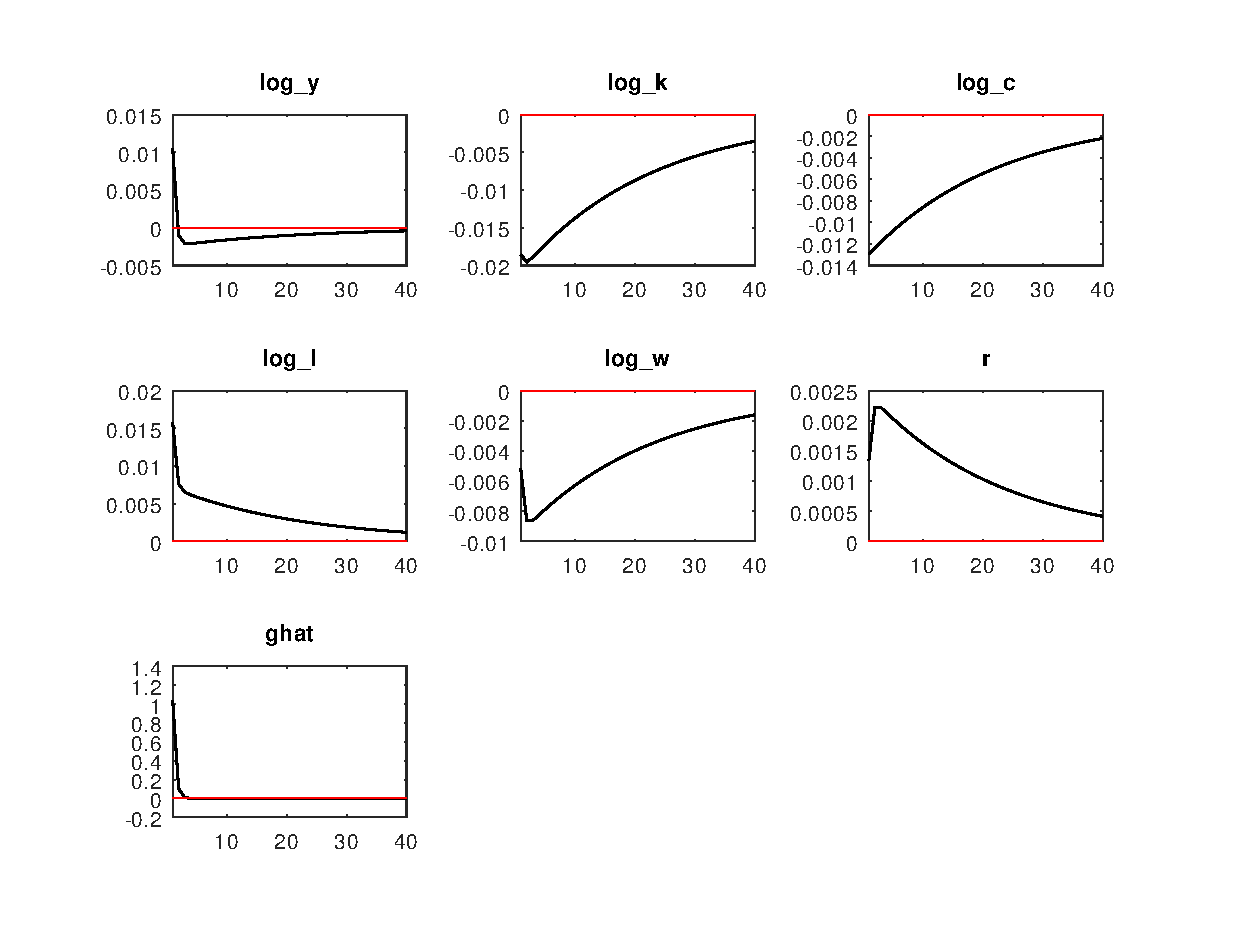
\includegraphics[width=0.80\textwidth]{RBCt_IRF_eps_g}
	\label{fig:rbcefectodynaregastotransitorio}
\end{figure}
\renewcommand{\rgcaptioneq}{\rgcaption{Efecto de un shock de gasto público transitorio en un modelo del ciclo real básico\footnote{Estimado con modelo RBC\_Baseline.mod de \href{https://github.com/JohannesPfeifer/DSGE_mod}{Repositorio de modelos DSGE en Dynare de Johannes Pfeifer.}}.}}
\begin{center}
	\rgcaptioneq
\end{center}


\begin{figure}[!htbp]
	\psfrag{log_y}[1][][0.5][0]{${\log(y)}$}
	\psfrag{log_k}[1][][0.5][0]{${\log(k)}$}
	\psfrag{log_c}[1][][0.5][0]{${\log(c)}$}
	\psfrag{log_l}[1][][0.5][0]{${\log(l)}$}
	\psfrag{log_w}[1][][0.5][0]{${\log(w)}$}
	\psfrag{r}[1][][0.5][0]{${r}$}
	\psfrag{A}[1][][0.5][0]{${A}$}
	\centering 
	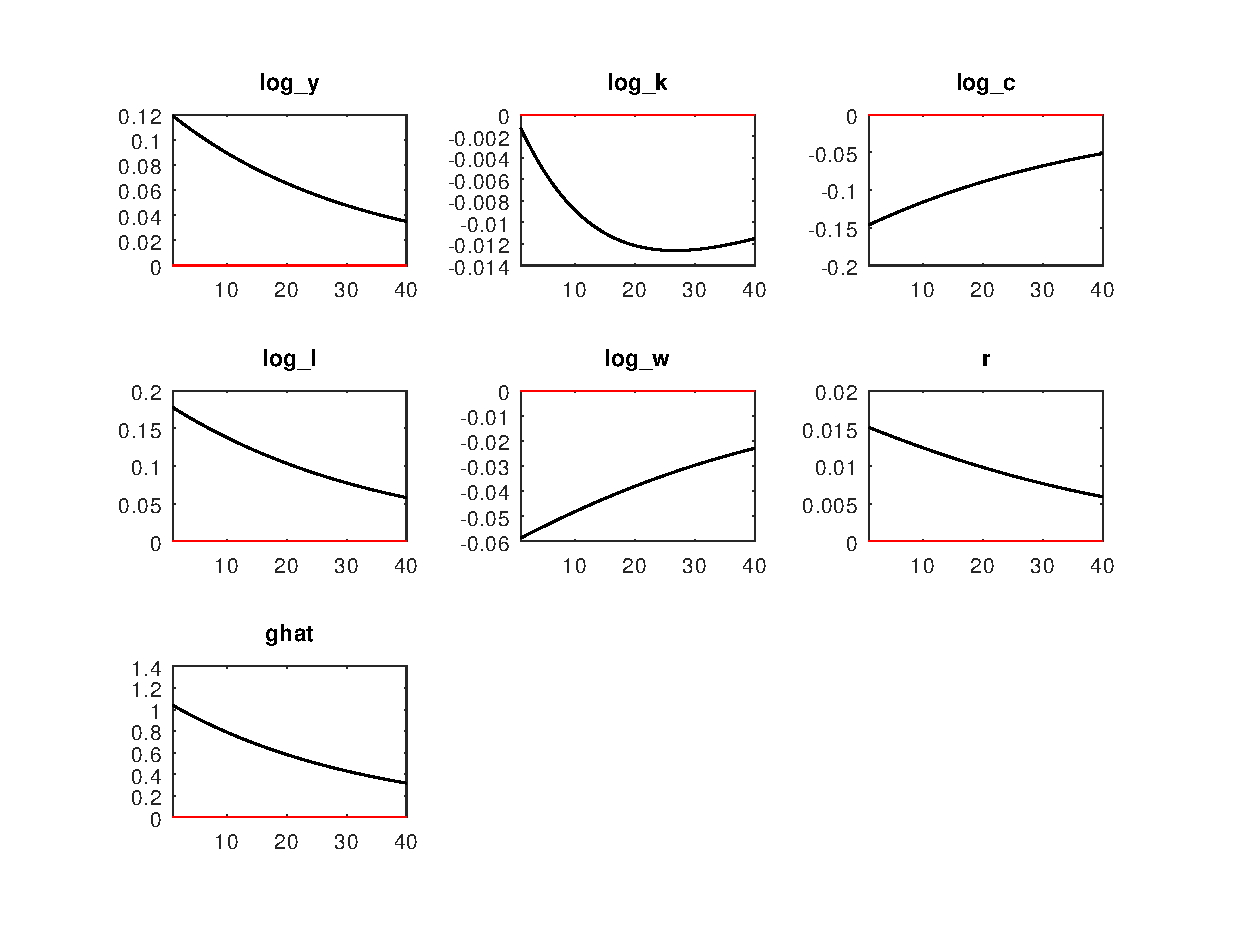
\includegraphics[width=0.80\textwidth]{RBCp_IRF_eps_g}
	
	\label{fig:rbcefectodynaregastopermanente}
\end{figure}
\renewcommand{\rgcaptioneq}{\rgcaption{Efecto de un shock de gasto público persistente en un modelo del ciclo real básico\footnote{Íbidem.}}}
\begin{center}
	\rgcaptioneq
\end{center}




\preguntas

\seccion{Test 2019}

\textbf{23.} Recientemente, los modelos neokeynesianos se han centrado en analizar los efectos de la política fiscal sobre el crecimiento. Señale la respuesta correcta:

\begin{itemize}
	\item[a] Una política fiscal expansiva en un país que forma parte de una Unión Monetaria tiene un efecto expansivo para la economía doméstica, aunque dependerá del grado acomodaticio de la política monetaria común.
	\item[b] Según esta escuela, ante una coyuntura de tipos de interés cero (\textit{zero lower bound}), el multiplicador del gasto público sería muy reducido (cercano a 0), lo que explicaría la baja o nula efectividad de la política fiscal.
	\item[c] Blanchard y Leigh (2013) encuentran que la consolidación fiscal llevada a cabo en varias economías avanzadas puede explicar tasas de crecimiento menores a las proyectadas ante unos multiplicadores fiscales durante el inicio de la crisis que alcanzaron valores superiores a 1.
	\item[d] Todas las anteriores son correctas.
\end{itemize}

\seccion{Test 2017}
\textbf{18.} Para que la política fiscal pueda suavizar las fluctuaciones económicas:

\begin{itemize}
	\item[a] Los gastos públicos deben ser siempre iguales a los ingresos públicos.
	\item[b] Los ingresos deben ser menores que los gastos si el PIB observado es mayor que el PIB potencial.
	\item[c] Los ingresos deben ser mayores que los gastos si el PIB observado es menor que el PIB potencial.
	\item[d] Ninguna de las anteriores.
\end{itemize}

\seccion{Test 2016}

\textbf{19.} La existencia de restricciones a la liquidez provoca:
\begin{itemize}
	\item[a] Que no se cumpla la equivalencia ricardiana.
	\item[b] Que el consumo del periodo sea poco sensible a las rentas del periodo.
	\item[c] Que el consumo del período no se vea afectado por las disminuciones de impuestos aunque éstas sean transitorias.
	\item[d] El traspaso de rentas futuras hacia el presente.
\end{itemize}

\textbf{27.} La curva de Laffer:
\begin{itemize}
	\item[a] Relaciona el nivel de presión fiscal de una economía con la inflación.
	\item[b] Implica que aumentos del tipo impositivo llevan a aumentos de la recaudación fiscal hasta alcanzar el tipo óptimo.
	\item[c] Implica que aumentos del tipo impositivo llevan necesariamente a reducciones más que proporcionales del crecimiento vía disminución de la renta disponible y el ahorro.
	\item[d] Implica que reduciendo el tipo impositivo por debajo del óptimo la recaudación fiscal puede aumentar.
\end{itemize}

\seccion{Test 2015}
\textbf{20.} Considere una economía intertemporal de dos períodos, $t$ y $t+1$, producción exógena, agentes idénticos, previsión perfecta y dos mercados, el mercado de bienes y el mercado de bonos. El agente representativo tiene una función de utilidad intertemporal:

\begin{equation*}
U(c_t, c_{t+1}) = \sqrt{c_t c_{t+1}}
\end{equation*}

Y dispone de una dotación de cuantía constante a lo largo de su vida. El gobierno de esta economía decide anunciar al principio del periodo $t$ la implantación de una política fiscal de presupuesto equilibrado en la que el gasto público será financiado íntegramente por un impuesto a tanto alzado. Más concretamente, el gobierno se plantea 2 posibles regímenes de política fiscal, A y B:

\begin{itemize}
	\item en el régimen A, $g_t = g$ y $g_{t+1} = 0$,
	\item en el régimen B, $g_t = 0$ y $g_{t+1} = g$,
	\item $g_s$, $s=t$, $t+1$, es el gasto público per cápita y $g>0$.
\end{itemize}

Dada la información disponible, y suponiendo que el anuncio del gobierno sea creíble, es posible afirmar que:

\begin{itemize}
	\item[a] El tipo de interés entre $t$ y $t+1$ será positivo en A, pero negativo en B.
	\item[b] El tipo de interés entre $t$ y $t+1$ será negativo en A, pero positivo en B.
	\item[c] El tipo de interés entre $t$ y $t+1$ será igual bajo los dos regímenes.
	\item[d] El tipo de interés entre $t$ y $t+1$ será negativo en A y negativo en B.
\end{itemize}

\seccion{Test 2014}

\textbf{23.} El teorema de la Equivalencia Ricardiana establece que, bajo ciertas condiciones:

\begin{itemize}
	\item[a] El aumento del gasto público supondrá una disminución del ahorro nacional en la misma cuantía.
	\item[b] Si el gobierno decide incrementar sus gastos, es irrelevante la manera en que lo financie.
	\item[c] El aumento del gasto público sólo permitirá aumentar la demanda agregada si se financia con un mayor endeudamiento.
	\item[d] Los países tienden a exportar aquellos bienes que fabrican con un coste relativamente más bajo respecto al mundo.
\end{itemize}

\seccion{Test 2013}
\textbf{15.} Considérese una economía intertemporal de tres períodos, $t$, $t+1$ y $t+1$, producción exógena, agentes idénticos, previsión perfecta y dos mercados, el mercado de bienes y el mercado de bonos. El agente representativo tiene una función de utilidad intertemporal:

\begin{equation*}
\ln c_t + \ln c_{t+1} + \ln c_{t+2}
\end{equation*}

y dispone de una dotación de cuantía constante a lo largo de su vida.

El gobierno de esta economía decide anunciar al principio del período $t$ la implantación de una política fiscal de presupuesto equilibrado en la que el gasto público será financiado íntegramente por un impuesto de tanto alzado. Más concretamente, el gobierno se plantea dos posibles regímenes de política fiscal, $A$ y $B$, definidos según la siguiente tabla:

\begin{center}
\begin{tabular}{l c c}
& Régimen A & Régimen B \\ \hline 
Período $t$ & $g_t = 0$ & $g_t = 0$ \\ \hline 
Período $t+1$ & $g_{t+1} = g$ & $g_{t+1} = g$ \\ \hline 
Período $t+2$ & $g_{t+2} = 0$ & $g_{t+2} = g$ \\ \hline
\end{tabular}
\end{center}

donde $g_s$, $s=t, t+1, t+2$ es el gasto público per cápita y $g >0$.

Dada la información disponible, y suponiendo que el anuncio del gobierno sea creíble, es posible afirmar que:

\begin{itemize}
	\item[a] El tipo de interés en $t+1$ no cambiaría con el régimen elegido.
	\item[b] El tipo de interés en $t+1$ sería más elevado bajo el régimen A.
	\item[c] El tipo de interés en $t+1$ sería más elevado bajo el régimen B.
	\item[d] Cualquiera de las respuestas anteriores podría ser correcta.
\end{itemize}

\seccion{Test 2011}
\textbf{14.} El supuesto de la equivalencia ricardiana implica que:
\begin{itemize}
	\item[a] Una disminución en los impuestos provoca un aumento instantáneo del consumo mientras que el ahorro permanece constante.
	\item[b] Una disminución en los impuestos provoca un aumento instantáneo en el ahorro, mientras que el consumo permanece constante.
	\item[c] Una disminución en los impuestos provoca un aumento en la renta permanente.
	\item[d] El efecto riqueza de una disminución en los impuestos es positivo.
\end{itemize}

\seccion{Test 2007}
\textbf{19.} Suponga que, en una economía, nadie se preocupa por el bienestar económico de las generaciones futuras. En este caso, la visión que proporciona la equivalencia Ricardiana sobre los efectos de una disminución de impuestos financiada con deuda, es:

\begin{itemize}
	\item[a] Totalmente inválida.
	\item[b] Totalmente válida porque el gobierno siempre tiene la opción de, a los pocos años, subir los impuestos para saldar la deuda.
	\item[c] Totalmente válida siempre y cuando el gobierno reduzca también su gasto.
	\item[d] Parcialmente válida porque muchos de los contribuyentes vivirán, y pagarán impuestos, durante un número sustancial de años tras el recorte de impuestos.
\end{itemize}

\notas

\textbf{2019} \textbf{23.} C

\textbf{2017:} \textbf{18.} D

\textbf{2016:} \textbf{19.} A \textbf{27.} B

\textbf{2015:} \textbf{20.} A

\textbf{2014:} \textbf{23.} B

\textbf{2013:} \textbf{15.} B

\textbf{2011:} \textbf{14.} B

\textbf{2007:} \textbf{19.} D

\bibliografia

Mirar en Palgrave:
\begin{itemize}
	\item budgetary policy
	\item built-in stabilizaers
	\item burden of the debt
	\item capital gains taxation
	\item economic growth
	\item economic growth in the very long run
	\item endogenous growth theory
	\item fine tuning
	\item fiscal and monetary policies in development countries
	\item fiscal multipliers
	\item fiscal stance
	\item fiscal theory of the price level
	\item forced saving
	\item full employment budget surplus
	\item functional finance
	\item government budget constraint
	\item government budget restraint
	\item growth and cycles
	\item individual retirement account
	\item infrastructure and growth
	\item long swings in economic growth
	\item monetary and fiscal policy overview
	\item neo-ricardian economics
	\item neo-Ricardianism
	\item new keynesian macroeconomics
	\item optimal fiscal and monetary policy (with commitment)
	\item optimal fiscal and monetary policy (without commitment)
	\item optimal savings
	\item over-saving
	\item pension systems: principles, debates and analytical errors
	\item pensions
	\item population ageing
	\item public debt
	\item public works
	\item retirement
	\item Ricardian equivalence theorem
	\item saving equals investment
	\item stabilization policy
	\item targets and instruments
	\item taxation of income
	\item taxation of wealth
	\item time consistency of monetary and fiscal policy
	\item vector autoregressions
\end{itemize}

Barro, R. (1974) \textit{Are government bonds net wealth?} Journal of Political Economy -- En carpeta del tema

Batini, N.; Eyraud, L.; Forni, L.; Weber, A. (2014) \textit{Fiscal Multipliers: Size, Determinants and Use in Macroeconomic Projections} IMF Fiscal Affairs Department -- Technical Notes and Manuals -- En carpeta del tema

Dolls, M.; Fuest, C.; Peichl, A. (2012) \textit{Automatic Stabilizers and Economic Crisis: US vs Europe} Journal of Political Economy -- En carpeta del tema

Gootzeit, M. J. (1987) \textit{Adam Smith of Balanced Budget Government Spending} History of Economics Society Bulletin -- En carpeta del tema

Groth (2017) \textit{Lecture notes in macroeconomics} Mimeo -- En carpeta del tema

Ramey, V. A. (2019) \textit{Ten Years After the Financial Crisis: What Have We Learned from the Renaissance in Fiscal Research?} Journal of Economic Perspectives: Spring 2019 -- En carpeta del tema

Sinn, H. W. (2000) \textit{Why a funded pension is useful and why it is not useful} NBER Working Paper Series -- En carpeta del tema

Sims, E. (2017) \textit{Graduate Macro Theory II: Fiscal Policy in the RBC Model} \url{https://www3.nd.edu/~esims1/fiscal_policy_sp2017.pdf} -- En carpeta del tema

\end{document}
